\documentclass[letterpaper,10pt]{article}

\usepackage{enumitem}
\usepackage{titling}
\usepackage{listings}
\usepackage{url}
\usepackage{hyperref}
\usepackage{setspace}
\usepackage{subfig}
\usepackage{sectsty}
\usepackage{pdfpages}
\usepackage{colortbl}
\usepackage{multirow}
\usepackage{multicol}
\usepackage{relsize}
\usepackage{amsmath}
\usepackage{wasysym}
\usepackage{fancyvrb}
\usepackage[yyyymmdd]{datetime}
\usepackage{amsmath,amssymb,amsthm,graphicx,xspace}
\usepackage[titlenotnumbered,noend,noline]{algorithm2e}
\usepackage[compact]{titlesec}
\usepackage{XCharter}
\usepackage[T1]{fontenc}
\usepackage[scaled]{beramono}
\usepackage[normalem]{ulem}
\usepackage{booktabs}
\usepackage{tikz}
\usetikzlibrary{arrows,automata,shapes,trees,matrix,chains,scopes,positioning,calc}
\tikzstyle{block} = [rectangle, draw, fill=blue!20,
text width=2.5em, text centered, rounded corners, minimum height=2em]
\tikzstyle{bw} = [rectangle, draw, fill=blue!20,
text width=4em, text centered, rounded corners, minimum height=2em]

\definecolor{namerow}{cmyk}{.40,.40,.40,.40}
\definecolor{namecol}{cmyk}{.40,.40,.40,.40}
\renewcommand{\dateseparator}{-}

\let\LaTeXtitle\title
\renewcommand{\title}[1]{\LaTeXtitle{\textsf{#1}}}

\lstset{basicstyle=\footnotesize\ttfamily,breaklines=true}

\newcommand{\handout}[5]{
	\noindent
	\begin{center}
		\framebox{
			\vbox{
				\hbox to 5.78in { {\bf ECE 350: Real-Time Operating Systems } \hfill #2 }
				\vspace{4mm}
				\hbox to 5.78in { {\Large \hfill #4  \hfill} }
				\vspace{2mm}
				\hbox to 5.78in { {\em #3 \hfill \today} }
			}
		}
	\end{center}
	\vspace*{4mm}
}

\newcommand{\lecture}[3]{\handout{#1}{#2}{#3}{Lecture#1}}
\newcommand{\tuple}[1]{\ensuremath{\left\langle #1 \right\rangle}\xspace}

\newcommand{\Rplus}{\protect\hspace{-.1em}\protect\raisebox{.35ex}{\smaller{\smaller\textbf{+}}}}
\newcommand{\Cpp}{\mbox{C\Rplus\Rplus}\xspace}


\addtolength{\oddsidemargin}{-1.000in}
\addtolength{\evensidemargin}{-0.500in}
\addtolength{\textwidth}{2.0in}
\addtolength{\topmargin}{-1.000in}
\addtolength{\textheight}{1.75in}
\addtolength{\parskip}{\baselineskip}
\setlength{\parindent}{0in}
\renewcommand{\baselinestretch}{1.5}
\newcommand{\term}{Spring 2023}
\newcommand{\termnumeric}{1235}

\singlespace


\begin{document}

\lecture{ 3 --- Sunrise to Sunset }{\term}{Jeff Zarnett}

\section*{Here When You Need Me}

We already learned about the lifecycle of a process, but the operating system itself has a lifetime as well. It needs to be started, it has a period where it executes, and will eventually shut down (for some reason or another). While it's running, it offers a number of services and a suite of functionality that is intended to make it easy and safe for user programs to execute.

\subsection*{Starting Up}
We will imagine the operating system is already installed on disk and not worry too much about systems without permanent storage (even though they did exist in the past). When you power on the computer, the CPU execution at a predetermined location. This is in the BIOS (Basic Input-Output System), which is firmware, when it's an older computer. Newer computers use  UEFI (Unified Extensible Firmware Interface) that stores the boot information on disk rather than in the firmware itself. I don't want to get too bogged down in the details about how this works, but however it's implemented, it goes to the configured boot device (usually a hard drive)  and starts execution of the boot loader. 

What's a boot loader? It's a small piece of code whose purpose is to start up the operating system. This may be a multi-stage process involving loading a progressively-larger boot program from disk, but in the end, the goal is to load the kernel and begin its execution. The boot loader program may do other things, like verify the state of the machine and if the diagnostics are okay, proceed; it can also initialize things like the CPU registers, device controllers, wipe memory...~\cite{osc}.

The boot loader itself has at least some initialization code located in the first block of the hard drive that is the boot device. If the system has more than one drive, not all of them are necessarily configured for booting the system. Only if the first block of the drive contains this information can it be used for booting. The actual boot loader might be bigger. No matter how many steps it takes, eventually control is transferred to the kernel itself and then it's running. 

Once the kernel is running, it can start the relevant operating system services, including the things that users will eventually interact with, like the login screen or the remote login server. Some services and utilities are always started when the OS begins running; others are configurable so that an administrator can choose to have them start on system boot up. Although they are started by the OS without any direct user interaction, most processes are still user-level programs that operate like normal and must interact with the OS through the system call interface. Speaking of...

\subsection*{What Can You Do For Me?}

The main purpose of the operating system is not to run itself, but is there to make things work for the user-level programs that are supposed to run. Our previous experience with systems programming has taught us a lot about the services that the operating system has to offer. Some examples of things we already asked the OS to do for us:
\begin{multicols}{2}
\begin{itemize}
	\item Process and thread creation, termination
	\item Inter-process communication
	\item Concurrency control
	\item Memory allocation
\end{itemize}
\end{multicols}

The operating system does a lot more than this, and the visibility of that functionality varies. The OS must check permissions whenever you want to open a file, but you probably do not notice or think about it unless somehow permission is denied. There is scheduling, which we had to think about when it comes to concurrency and synchronization, but it was treated as external forces and nothing we could control. And then there are yet other things that the operating system does independently and we may or may not have any way of interacting with them, like the accounting and record keeping the system does.

A visual representation of that from~\cite{osc}:
\begin{center}
	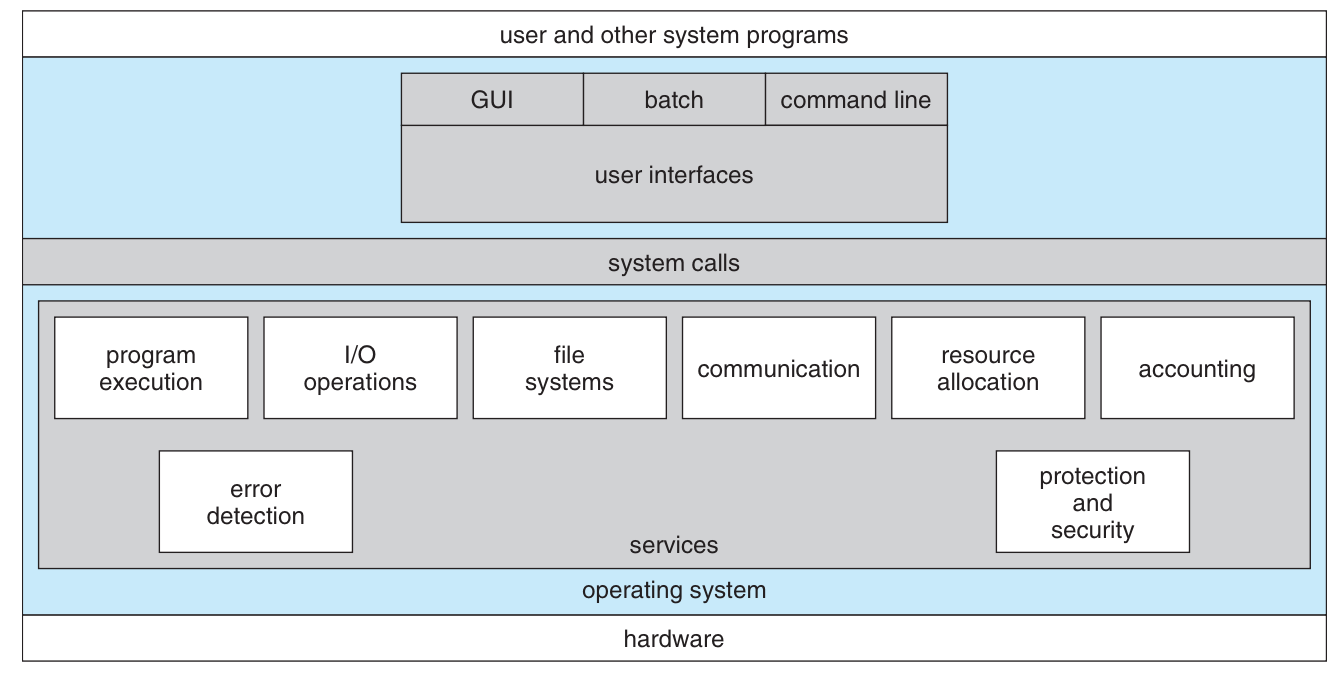
\includegraphics[width=0.75\textwidth]{images/os-structure.png}
\end{center}

At steady-state, the operating system runs whatever background tasks it needs to do, but the interesting things happen as the result of a user-level program asking for the OS to do something. And you know how that works...

\paragraph{Remember, it's a Trap.}

Previously, we covered this from the point of view of a user program that wants to activate the kernel. We said that it operates on interrupts and the interesting thing is the intentional use of the trap: this is how a user program gets the operating system's attention. When a user program is running, the operating system is not; we might even say it is ``sleeping''. If the program running needs the operating system to do something, it needs to wake up the OS: interrupt its sleep. When the trap occurs, the interrupt handler (part of the OS) is going to run to deal with the request.

We saw the concept of user mode vs. supervisor mode instructions: some instructions are not available in user mode. Supervisor mode, also called kernel mode, allows all instructions and operations. Even something seemingly simple like reading from disk or writing to console output requires privileged instructions. These are common operations, but they involve the operating system every time.

Modern processors keep track of what mode they are in with the mode bit. This was not the case for some older processors and some current processors have more than two modes, but we will restrict ourselves to dual-mode operation with a mode bit. Thus we can see at a glance which mode the system is in. At boot up, the computer starts up in kernel mode as the operating system is started and loaded. User programs are always started in user mode. When a trap or interrupt occurs, and the operating system takes over, the mode bit is set to kernel mode; when it is finished the system goes back to user mode before the user program resumes~\cite{osc}.

Suppose a text editor wants to output data to a printer. Management of I/O devices like printers is the job of the OS, so to send the data, the text editor must ask the OS to step in, as in the diagram below:

\begin{center}
	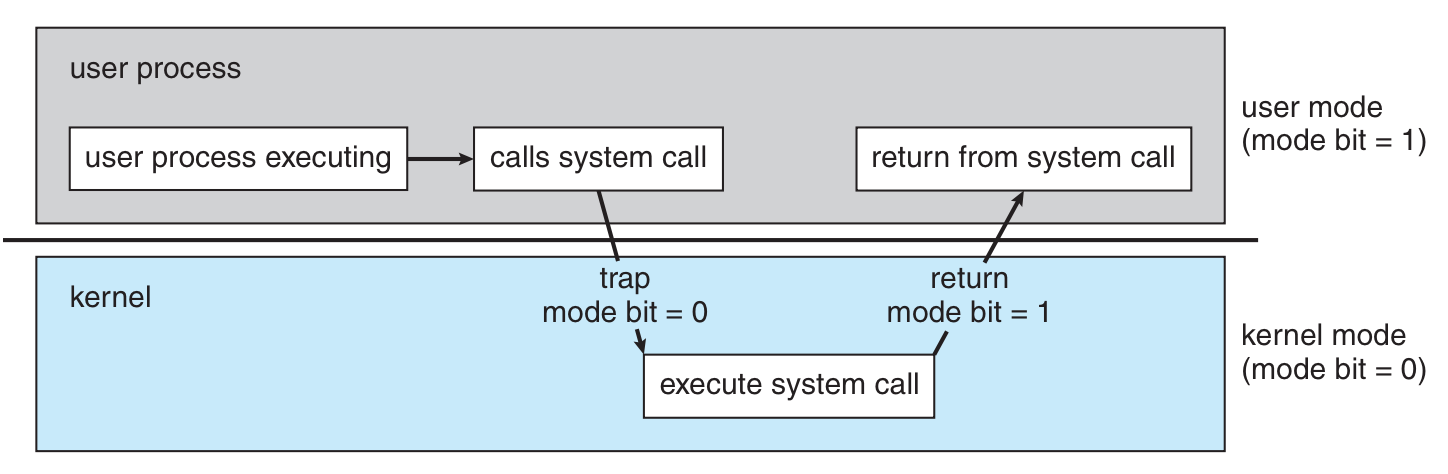
\includegraphics[width=0.75\textwidth]{images/trap.png}\\
	Transition from user to supervisor (kernel) mode~\cite{osc}.
\end{center}

So to print out the data, the program will prepare the data for printing. Then it calls the system call. You may think of this as being just like a normal function call, except it involves the operating system. This triggers the operating system (with a trap). The operating system responds and executes the system call and dispatches that data to the printer. When this job is done, operation goes back to user mode and the program returns from the system call.

\paragraph{Motivation for Dual Mode Operation.}

Why do we have user and supervisor modes, anyway? As Uncle Ben told Spiderman, ``with great power comes great responsibility''. Many of the reasons are the same as why we have user accounts and administrator accounts: we want to protect the system and its integrity against errant and malicious users.

An example: multiple programs might be trying to use the same I/O device at once. If Program~1 tries to read from disk, it will take time for that request to be serviced. During that time, if Program~2 wants to read from the same disk, the operating system will force Program~2 to wait its turn. Without the OS to enforce this, it would be up to the author(s) of Program~2 to check if the disk is currently in use and to wait patiently for it to become available. That may work if everybody plays nicely, but without someone to enforce the rules, sooner or later there will be a program that does something nasty, like cancel another program's read request and perform its read first.

This doesn't come for free, of course: there is a definite performance trade-off. Switching from user mode to kernel mode requires some instructions and some time. It would be faster if everything ran in kernel mode because we would spend no time switching. Despite this, the performance hit for the mode switch is judged worthwhile for the security and integrity benefits it provides.

\paragraph{Policy and Mechanism.}
On this subject of the motivation for dual mode operation, let's talk a little bit about policy and mechanism. In short, \textit{policy} tells us what will be done and \textit{mechanism} is how the policy is carried out; ideally these are separated to some degree to provide flexibility~\cite{osc}.  

Some policies are configurable, such as how much do priorities of processes matter; others are not, such as whether processes can read from files for which they do not have the read-permission. What is configurable policy is a question of operating system design. Actually applying the policy is involves both design and implementation. For the most part, though, operating systems tend to err on the side of having fewer configuration options. Is that because the authors know best what the user (system administrator) wants and needs, because they merely think they do? That's a lengthy debate, to be sure, but outside the scope of this course.

From the point of view of the user program, policy is something that we have to contend with but may not have any say in it, though you could hypothetically require that the application be granted certain permissions before running. If the policy is that it's not possible to access the memory of other processes, well, that's policy and we have to write a program with that in mind. Having to follow the rules may be less convenient, but it's not optional.

The operating system code itself has no such restrictions: it is free to ignore policy if it wants and freely read and write in memory. This level of access requires that the operating system be, to some great extent, trusted by the application authors. If you didn't trust the operating system, would you feel comfortable logging in to online banking on that system? Are you sure?

The operating system also has to be responsible for the mechanism: enforcement of the policy. We will see in later topics how to enforce certain policies, such as fairness in terms of CPU time, or terminating a thread if it tries to read memory that belongs to some other process. 

\subsection*{Switching Processes or Threads}
We discussed some details about how a process switch occurs and reviewed it recently, but there wasn't much detail on when does a switch of processes happen? From the point of view of the application program we say that the process switch could happen at any time and we tried to imagine that it would happen at the most inconvenient time to cause an issue. It could happen at any time from the point of view of the user program, but the operating system gets to choose (to some extent) when it happens. The operating system, fortunately, does get to choose which process will run next, but that's not a trivial decision, to the point where scheduling is one of the major topics of this course.

Realistically, processes always get paused as a result of an interrupt, and that may or may not result in a thread switch. Some of them are intentional, voluntary invocations of system calls which result in the trap interrupt. Other interrupts, regardless of source, lead to the same thing. The interrupt is handled and while that's the case, the operating system is running and the thread that was executing before is suspended. 

The first situation where a process (thread) switch must occur is when the currently-executing process (thread) gets blocked. It's the user program that chose to wait for network data or reading from a file. Whatever the reason that the current process becomes blocked, that means it cannot continue executing.

Similarly, another reason that process switch must occur is the termination (voluntary or otherwise) of the currently-executing process or thread. If it was a call to voluntarily exit, that was a system call. If it occurred as a result of something going wrong (e.g., division by zero), that's an exception and the exception is an interrupt.

That covers the mandatory switches but there are those where the operating system chooses to switch. Whatever interrupt has been handled, whether a system call trap, the currently-executing thread is suspended and the operating system is running. After dealing with the request (whether or not a final answer is ready), it's equally valid to restore a different process to run next rather than the one that was just suspended. This is, again, a scheduling decision. But this category covers a lot of situations, including creating a new process.

When we get to scheduling, we'll also consider things like wanting to prevent monopolization of the CPU through various mechanisms that force threads to take turns. One possible way to do so is a timer interrupt, where an interrupt is generated after a period of time, and that's a prompt to consider if a switch should occur.

\subsection*{Keeping Track}
At steady state, the operating system will have to keep track of the various resources in some sort of tables or other data structures such as memory tables, I/O tables, file tables, and process tables~\cite{osi}. We will get into the details of how memory, I/O, and files are managed in later topics. But they are pretty much exactly what they sound like.  But let's cover these at a high level now.

Memory tables track the state of memory, both the memory that's free and what is in use. The operating system needs memory for itself to do its job, such as containing the process control blocks, buffers, etc. And unlike a user process that can ask the OS to allocate and deallocate memory for it, the OS has to do this the ``hard'' way. But in addition to that, the OS needs to keep track of some attributes of memory, including the protection rules and whether any sections of memory are shared~\cite{osi}. 

Memory tables may need to be updated every time memory is allocated or deallocated and whenever changes take place on shared memory. Process creation and destruction also result in significant changes to the memory being managed as well as the process. Yes, a new process control block needs to be created, but also the memory space for the process itself is required -- the program has some global variables, stack, and heap.

I/O tables are used for keeping track of the status of the various I/O devices attached to the system. I/O devices may be shared or assigned to a specific process. But more importantly, when there are I/O operations in progress, it's necessary to keep track of what the operation is and where the data is coming from and going to. 

And then there are file tables: the operating system keeps track of which files are open overall, and which ones a given process is using. Remember that in UNIX, the abstraction is that everything is a file, so files refer to not only actual files on disk but also other things like sockets or pipes.


\subsection*{Shutting Down}
Shutting down the operating system is relatively straightforward procedure. To do so, it will need to notify all running processes that they should exit. Sending them a signal that asks them to exit should be sufficient, and ideally the program authors have implemented something that makes it a graceful shutdown rather than just dying unceremoniously. 

As you may know, asking the programs to shut down politely may not actually get them to terminate. This may be because they intentionally or unintentionally ignore the polite request to terminate. If you're editing a document, the editor might have a little pop up window asking if you'd like to save changes, and will wait an indefinite period for the user to decide. If the OS shutdown has been called, at some point you may decide to forcibly terminate the processes even if it means the user loses some work. It's an interesting design decision to think about how long you are willing to wait. 

The other consideration is: can every user, even those who are not administrators, request a shutdown of the system? For a desktop system then it is probably fine -- if I'm done with the computer and want to turn it off to save power that's sensible. But if it's a multi-user server, other people would be very annoyed if I turned it off while they are using it!

Once the user programs are all terminated, the operating system can terminate its own internal services and then signal to the hardware to switch the machine off, or, alternatively, to restart. And if we choose restart, then it's back to the beginning.

\bibliographystyle{alphaurl}
\bibliography{350}


\end{document}